\documentclass{article}

% preambulo:
\input{control_tpf_preamble.tex}

\begin{document}

\newgeometry{} % margenes default para la caratula
% caratula:
\input{control_tpf_caratula.tex}


% cambio los margenes para el resto del documento
\newgeometry{top=2.5cm, bottom=2.0cm, left=2.25cm, right=2.25cm}

% indice:
\tableofcontents
\newpage


\section{Introducción}

En el presente trabajo práctico se implementó un sistema para simular el control aerodinámico similar a un helicóptero, es decir con 2 DOF (dos grados de libertad), sobre una base fija.\par
El montaje del sistema se realizó de manera artesanal, sobre un taller propio con los elementos disponibles, y el control digital se implementó utilizando un Arduino.\\

\begin{figure}[H]
\centering
\includegraphics[width=0.7\linewidth]{images/modFinal2.jpg}
\caption{Simulador de sistema aerodinámico de helicóptero - Versión final}
\end{figure}

\newpage

\section{Análisis del sistema}
\subsection{Factores externos - Montaje}

Previo al planteo del sistema mecánico, se analizan los factores que afectarían al libre movimiento del mismo. Para dar el movimiento se incorporaron dos motores del estilo utilizado en drones, en este caso de hasta 25000 RPM.\\
La barra horizontal de madera sobre la que se montan ambos motores se la considera como una masa, la cual producirá una fuerza en oposición a la que traten de realizar los motores. Esto ya sea para el movimiento vertical (Pitch) u horizontal (Yaw). Para sujetar los motores se utilizaron dos bridas de plástico.\\
Por el centro de dicha barra de madera se hace pasar una barra de metal liviano, que actuará de eje vertical para que la barra de madera pueda rotar libremente.\\

\begin{figure}[H]
\centering
\includegraphics[width=0.3\linewidth]{images/rotor.jpg}
\caption{Barra de madera y eje}
\end{figure}

Esta barra de metal, en uno de sus extremos tiene colocado un potenciómetro (para poder tomar medición de la posición), y en el otro un ruleman para que el movimiento sea mas suave. Dicho ruleman se lo representará como un rozamiento vizcoso.\\
La barra de metal va colocada sobre sus extremos a un soporte en forma de 'U', sobre el cual van colocados el potenciómetro y ruleman mencionados previamente. El soporte en forma de 'U' está realizado sus laterales en madera, y la base sobre un perfil de aluminio. Esta pieza se la modelará como una masa.\\ En su centro, se colocó una pieza de ajuste para poder, mediante un tornillo y tuerca, unirlos a otro ruleman en la parte inferior, para dar un movimiento horizontal suave.\\

\begin{figure}[H]
\centering
\includegraphics[width=0.3\linewidth]{images/preMontaje.jpg}
\caption{Modelo semiterminado}
\end{figure}

Finalmente, debajo de dicha pieza, adosado al tornillo se colocó otro potenciómetro, para poder medir el movimiento horizontal. 

\begin{figure}[H]
\centering
\includegraphics[width=0.4\linewidth]{images/base.jpg}
\includegraphics[width=0.4\linewidth]{images/baseU.jpg}\caption{Base y pieza de ajuste}
\end{figure}

\begin{figure}[H]
\centering
\includegraphics[width=0.4\linewidth]{images/poteBase1.jpg}
\includegraphics[width=0.4\linewidth]{images/poteBase2.jpg}\caption{Base agujereada y potenciómetro colocado}
\end{figure}

El conjunto queda apoyado sobre una base de madera, ajustando la pieza circular de ajuste con dos tornillos.

\begin{figure}[H]
\centering
\includegraphics[width=0.4\linewidth]{images/modPrevio.jpeg}
\caption{Modelo terminado}
\end{figure}

\subsection{Sistema mecánico}
Teniendo los factores constructivos previamente mencionados, se procede a realizar el modelo mecánico. Para simplificar el análisis, como se observará luego el movimiento sobre ambos ejes por separado, se modelan dos sistemas.\par
Tomando el caso del sistema para regular el Pitch, se considera por un lado el momento de inercia de los motores más el de la barra de madera y la de metal (que hace de eje). Ambos está sometidos a un cierto roce dado por el ruleman y el eje del potenciómetro (dado que están adosados). Y también a una cierta elasticidad producida por los cables al intentar girar de extremo a extremo. Esto puede modelarse como sigue:

\begin{figure}[H]
\centering
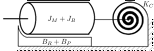
\includegraphics[width=0.8\linewidth]{images/modelPitch.png}
\caption{Modelo mecánico para el sistema de Pitch}
\end{figure}

Del cual se puede obtener la función transferencia de segundo orden entre el torque producido por el motor y el ángulo de gior (Pitch). Considerando J como el conjunto de los momentos de inercia y B para el rozamiento total:

\[
T_M = J \cdot \ddot{\theta_P} + B \cdot \ddot{\theta_P} + K_C \cdot \theta_P
\]

\[
T_M = J \cdot \theta_P \cdot S^2 + B \cdot \theta_P \cdot S + K_C \cdot \theta_P
\]

\[
\frac{\theta_P}{T_M} = \frac{1}{J \cdot S^2 + B \cdot S + K_C}
\]

Para el caso de Yaw, se puede modelar de manera similar. Se tienen los momentos de inercia del otro motor, más el de la barra de madera con su eje y se añade la 'U'. Esta esta sometida en su eje al roce dado por el otro ruleman y el otro potenciómetro para medir posición. Por otra parte también es modificada por una cierta elasticidad dada por los cables de interconexión, que como se verá más adelante afectarán al movimiento horizontal. Teniendo esto en cuenta, el modelo a utilizar es similar, con las variables correspondientes:

\begin{figure}[H]
\centering
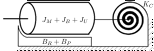
\includegraphics[width=0.8\linewidth]{images/modelYaw.png}
\caption{Modelo mecánico para el sistema de Yaw}
\end{figure}

Del cual se puede obtener la función transferencia entre el ángulo de rotación y el torque producido por el motor:

\[
T_M = J \cdot \ddot{\theta_Y} + B \cdot \ddot{\theta_Y} + K_C \cdot \theta_Y
\]

\[
T_M = J \cdot \theta_Y \cdot S^2 + B \cdot \theta_Y \cdot S + K_C \cdot \theta_Y
\]

\[
\frac{\theta_Y}{T_M} = \frac{1}{J \cdot S^2 + B \cdot S + K_C}
\]

\newpage

\section{Implementación en Arduino}

Para realizar el control digital, se utilizó un Arduino Uno, más la placa Puente H con L298 provista también por dicho fabricante para el control de los motores. Esto último fue necesario dado que ambos motores juntos en máxima potencia llegan a 1.5A de consumo total aproximadamente.\par
Los potenciómetros de posición, más los de ajuste manual y las entradas de señal externas para efectuar mediciones se conectaron a las entradas ADC del Arduino. Para el control del Puente H, se utilizaro otras 6 salidas digitales (3 para cada motor).\par
Se utilizó en principio un control proporcional derivativo (PD, para tener una respuesta más rápida del sistema). Pero dado que posee mucho error permanente (como se explicará luego), se añadió control integrativo, teniendo finalmente un control PID. Para hallar las constantes, el método utilizado consiste en anular KD y KI, y comenzar a aumentar KP hasta que el sistema comience a oscilar. Luego se setea la mitad del valor oscilatorio, y se aumenta KD para mejorar el tiempo de respuesta del sistema. Finalmente, se ajusta KI para eliminar el error permamente. Esto se realizó para cada sistema, es decir primero para el Pitch, y luego para el Yaw.\par 



\newpage

\section{Placa de interconexionado}

\subsection{Interfaces}

Para facilitar el conexionado al Arduino, se realizó una placa que actúa de interfaz entre este y el resto del sistema. Sobre ella se facilitan los siguientes elementos:

\begin{itemize}
\item Dos potenciómetros para poder realizar por un lado un control manual del Pitch, y por otro del Yaw.
\item Un conector polarizado para el potenciómetro que mide Pitch, y otro para el que mide Yaw.
\item Un conector polarizado para ingresar una señal externa para ajustar el Pitch, y otro para la señal de Yaw (más un jumper para puentearlas si se desea tener la misma señal para ambos).
\item Dos puntos de prueba para medir los valores de los potenciómetros con el osciloscopio.
\item Un conector polarizado para ingresar con la fuente externa para el Puente H.
\item Conectores polarizados para conectar los motores desde ésta placa hacia el Puente H.
\item Conectores polarizados para conectar las señales de control (PWM y las dos que determinan el sentido de giro) desde ésta placa hacia el Puente H.
\end{itemize}

\subsection{Modelo PCB}

\begin{figure}[H]
\centering
\includegraphics[width=0.4\linewidth]{images/cobre.png}
\includegraphics[width=0.4\linewidth]{images/componentes.png}\caption{PCB - Lado Cobre y Componentes}
\end{figure}

\newpage

\section{Mediciones}

\subsection{Pitch - Respuesta al escalón}

Para observar el tiempo de respuesta del sistema, se ingresó con una señal cuadrada de 0.1Hz a las entradas de control manual de Pitch y Yaw, en experimentos separados.\\

\begin{figure}[H]
\centering
\includegraphics[width=0.8\linewidth]{images/escalonPitch.jpeg}\caption{Medición de Pitch - Respuesta al escalón}
\end{figure}

Se tiene a partir de la medición de extremo a extremo que el tiempo para establecerse al subir es de aproximadamente 1 segundo, y posee un pequeño amortiguamiento donde se acomoda al punto seteado (dado que se pasó un poco). El movimiento tiene una pendiente suave, dado que el peso de la barra está en oposición a éste.

\begin{figure}[H]
\centering
\includegraphics[width=0.8\linewidth]{images/escalonInversoPitch.jpeg}\caption{Medición de Pitch - Respuesta al escalón}
\end{figure}

En el caso de la bajada, ésta resulta más abrupta, dado que el peso de la barra de madera contribuye en esa dirección. Al igual que en la subida, se pasa un poco del punto seteado y vuelve a subir un poco para alinearse.

\subsection{Yaw - Respuesta al escalón}


\begin{figure}[H]
\centering
\includegraphics[width=0.8\linewidth]{images/escalonYaw.jpeg}\caption{Medición de Yaw - Respuesta al escalón}
\end{figure}

Se tiene a partir de la medición de extremo a extremo que, en este eje afecta más la inercia de la estructura en forma de 'U', obteniendo un tiempo de respuesta de aproximadamente 2 segundos. En este caso la hélice gira en el sentido normal, es decir en favor de su curvatura.

\begin{figure}[H]
\centering
\includegraphics[width=0.8\linewidth]{images/escalonInversoYAW.jpeg}\caption{Medición de Yaw - Respuesta al escalón}
\end{figure}

En este caso, se obtiene una respuesta más lenta, dado que la hélice gira en sentido opuesto al normal, es decir en contra de su curvatura. Esto produce que el empuje máximo que puede generar es menor. Notar que le demanda casi todo el período llegar a establecerse en el punto de seteo.

\newpage

\section{Conclusiones}

A partir de efectuar varias pruebas se pudieron observar tanto puntos a favor como limitaciones del diseño.\par
Por un lado, en el caso del giro horizontal (Yaw), además de la limitación del sentido de giro de la hélice, la estructura ofrece mayor inercia en comparación a la barra de madera para el movimiento vertical (Pitch). Puede mejorarse esto con motores de mayor cantidad de RPM, y de ser posible con hélices que admitan giro en ambos sentidos por igual.\par
Ambos movimientos resultaban también afectados por los cables de conexión para los motores y el potenciómetro de medición de Pitch, dado su grosor. Una manera de mejorar esto es utilizar cables más blandos/finos, dado que los motores no poseen un gran consumo de corriente.\par
Por otra parte, el tamaño reducido y los rulemanes permiten en general que la estructura tenga un movimiento suave en ambos ejes, teniendo como topes únicamente los límites de los potenciómetros. Para un setpoint fijo, se observó que el sistema alcanza rápidamente el punto de equilibrio si se lo desbalancea manualmente.

\newpage

\section{Bibliografía}
\begin{itemize}
\item Idea para la maqueta: https://www.quanser.com/products/quanser-aero/
\item Funcionamiente básico y conexiones de la placa Puente H: https://www.prometec.net/l298n/ 
\item Motores con hélices: https://monarcaelectronica.com.ar/productos/motor-con-helice-12x20mm-dc-37v-25000rpm-mona/
\item Control PID Digital (Apuntes de clase)
\end{itemize}
\end{document}
